%% Additional tables of the replication package (not part of the paper or its
%% supplementary material). Build: pdflatex replication_tables.tex
\documentclass[a4paper,10pt]{article}
\usepackage[margin=2cm]{geometry}
\usepackage[T1]{fontenc}
\usepackage{lmodern}
\input{glyphtounicode}\pdfgentounicode=1
\usepackage{booktabs,multirow,xcolor,adjustbox,caption,amsmath,url,graphicx,xspace}
\usepackage{xr}\externaldocument{main}   % table captions refer to sections of the paper
\renewcommand{\thetable}{R\arabic{table}}
\renewcommand{\thefigure}{R\arabic{figure}}
\captionsetup{font=small,labelfont=bf}
\setlength{\parindent}{0pt}
\setlength{\parskip}{4pt}
\begin{document}
\begin{center}
{\Large\bfseries Replication package: additional tables}\\[4pt]
Mono-fix or Poly-fix? Bug Fixes Beyond the Main Language and Their Effect on Bug Localization\\[2pt]
A Eashaan Rao and Sridhar Chimalakonda
\end{center}

This document belongs to the replication package
(\url{https://github.com/eashaan-rao/polyglot-bug-localization}). It holds
tables needed to reproduce or inspect the runs that are neither in the paper
nor in its supplementary material.

\textbf{Data details.} Candidate files are the text files of the pre-fix
snapshot (at most 1\,MB, no NUL byte in the first 8\,KB); the universe R keeps
those the classification ruleset counts (median 1{,}890 files in localstack to
21{,}658 in elasticsearch per snapshot) and the text universe T all text files
(robustness condition R3). Fold~1 has 719 primary-anchored test bugs (483 Mono-fix, 213
Poly-fix, 23 multi-language only outside the broad grain), fold~2 has 718 (505,
206, 7); bugs whose fixed files were all added by the fix are left out of the
rank metrics, leaving 1{,}399 Mono-fix and Poly-fix test bugs. The 1{,}226
filter-excluded reports are distributed as elasticsearch 363, airflow 383,
ansible 295, dolphinscheduler 83, localstack 63 and liquibase 39. BeetleBox has
more C++ and JavaScript bugs (5{,}268 and 3{,}783) than Java or Python bugs
(3{,}707 and 3{,}759).

\begin{table*}[t]
\caption{Positioning: what each line of work provides and what this study adds.}
\label{tab:positioning}
\small
\begin{adjustbox}{max width=\linewidth}\begin{tabular}{p{3.3cm}p{6.2cm}p{6.6cm}}
\toprule
Line of work & Strength we use & Gap this study addresses \\
\midrule
Fix characterisation & Method for classifying fixes; multi-hunk taxonomy & Classifies by size and distance, not by file type \\
Cross-language BL (BLAZE, BeetleBox) & Multi-language ground truth; language-agnostic technique & Unit is a single-language fix within a project \\
Language-interaction bugs (xLoc) & Bugs at language boundaries & Bugs \emph{caused} by a boundary, not fixes that \emph{cross} one \\
Dataset quality & Ground truth affects measured performance & Concerns files wrongly included, not files fixes contain \\
Polyglot SE / RTS & Monolingual tools can be unsafe on polyglot code & Different task (testing, not localization) \\
LLM-based localization (agents, rankers) & Current techniques; graph-based tools; retrieve-and-rerank & Evaluated on source-only targets (SWE-bench, LocBench) \\
\bottomrule
\end{tabular}\end{adjustbox}
\end{table*}

% generated by Scripts/analysis/paper_tables.py -- do not edit
\begin{table*}[t]
\caption{Learning rate selected on validation MAP (seed 13) and, in parentheses, the selected epoch / epochs run before early stopping (BLAZE at most 15, FLIM at most 10).}
\label{tab:lr}
\footnotesize
\begin{adjustbox}{max width=\linewidth}\begin{tabular}{lllll}
\toprule
 & \multicolumn{2}{c}{BLAZE} & \multicolumn{2}{c}{FLIM} \\
\cmidrule(lr){2-3}\cmidrule(lr){4-5}
Project & fold 1 & fold 2 & fold 1 & fold 2 \\
\midrule
elasticsearch (J) & $2{\times}10^{-5}$ (1/4) & $2{\times}10^{-5}$ (4/7) & $2{\times}10^{-5}$ (2/5) & $2{\times}10^{-5}$ (6/9) \\
liquibase (J) & $2{\times}10^{-7}$ (15/15) & $2{\times}10^{-6}$ (8/11) & $5{\times}10^{-5}$ (6/9) & $2{\times}10^{-5}$ (3/6) \\
dolphinscheduler (J) & $2{\times}10^{-6}$ (12/15) & $2{\times}10^{-7}$ (11/14) & $5{\times}10^{-5}$ (2/5) & $2{\times}10^{-5}$ (9/10) \\
ansible (P) & $2{\times}10^{-5}$ (1/4) & $2{\times}10^{-7}$ (12/15) & $5{\times}10^{-5}$ (3/6) & $5{\times}10^{-5}$ (5/8) \\
airflow (P) & $2{\times}10^{-5}$ (1/4) & $2{\times}10^{-5}$ (1/4) & $2{\times}10^{-5}$ (3/6) & $2{\times}10^{-5}$ (6/9) \\
localstack (P) & $2{\times}10^{-7}$ (14/15) & $2{\times}10^{-7}$ (15/15) & $5{\times}10^{-5}$ (2/5) & $2{\times}10^{-5}$ (7/10) \\
\bottomrule
\end{tabular}\end{adjustbox}
\\[2pt]{\footnotesize Training and scoring cost on one NVIDIA L40 (all seeds): BLAZE: 18 runs, 74 GPU-hours; BLAZE-all: 6 runs, 13 GPU-hours; FLIM: 18 runs, 14 GPU-hours.}
\end{table*}


\begin{table}[t]
\caption{Reachability of ground-truth files in the test sets, before any technique is run (fold~1; fold~2 in parentheses).}
\label{tab:reach}
\small
\setlength{\tabcolsep}{3pt}
\begin{adjustbox}{max width=\linewidth}\begin{tabular}{lrr}
\toprule
 & Mono-fix & Poly-fix \\
\midrule
Test bugs & 483 (505) & 213 (206) \\
Ground-truth files per bug, mean & 2.3 (2.5) & 4.4 (4.2) \\
Bugs with an added (unreachable) file & 8.7\% (7.7\%) & 34.7\% (33.0\%) \\
GT files parseable & 99.9\% (100\%) & 62.8\% (65.8\%) \\
Bugs with $\ge$1 parseable GT file & 100\% (100\%) & 98.1\% (98.5\%) \\
Bugs with only parseable GT files & 99.8\% (100\%) & 10.8\% (10.2\%) \\
\bottomrule
\end{tabular}\end{adjustbox}
\end{table}

% generated by Scripts/analysis/paper_tables.py -- do not edit
\begin{table}[pos=t]
\caption{Where the Poly-fix penalty comes from (both folds). MRR of Mono-fix and Poly-fix bugs; MAP of Mono-fix bugs and of the primary-language and the secondary-language ground-truth files of Poly-fix bugs, each subset ranked with the other ground-truth files of the bug removed (the convention of Figure~\ref{fig:decomp}).}
\label{tab:decomp}
\footnotesize
\setlength{\tabcolsep}{2.4pt}
\begin{adjustbox}{max width=\linewidth}\begin{tabular}{lrrrrr}
\toprule
 & \multicolumn{2}{c}{MRR} & & \multicolumn{2}{c}{MAP, Poly-fix} \\
\cmidrule(lr){2-3}\cmidrule(lr){5-6}
Technique & Mono & Poly & MAP Mono & primary & secondary \\
\midrule
BM25 & .389 & .436 & .311 & .291 & .203 \\
FLIM-strict & .466 & .513 & .370 & .395 & n/a \\
FLIM-fallback & .462 & .511 & .365 & .383 & .055 \\
BLAZE & .329 & .396 & .255 & .286 & .142 \\
LocAgent$^{a}$ & .687 & .635 & .456 & .432 & .000 \\
SweRank$^{b}$ & .714 & .686 & .477 & .468 & .001 \\
SweRank, retriever only$^{b}$ & .630 & .570 & .415 & .389 & .001 \\
Random ranking & .004 & .009 &  &  &  \\
\bottomrule
\end{tabular}\end{adjustbox}
\\[2pt]{\footnotesize $^{a}$Python projects, AP@10 and RR@10. $^{b}$Python projects.}
\end{table}

% generated by Scripts/analysis/paper_tables.py -- do not edit
\begin{table*}[t]
\caption{RQ3 for the two techniques built on language models, which run on the Python projects only: MAP (AP@10 for LocAgent) of Mono-fix and Poly-fix test bugs per project (both folds) and Cliff's $\delta$ of Poly-fix against Mono-fix ($^{*}$: Holm-adjusted Mann--Whitney $p<0.05$). BM25 on the same bugs for reference. The last row is the adjusted class effect as in Section~\ref{sec:analysis}.}
\label{tab:rq3py}
\footnotesize
\setlength{\tabcolsep}{2.6pt}
\begin{adjustbox}{max width=\linewidth}\begin{tabular}{lr rrr rrr rrr rrr}
\toprule
 & & \multicolumn{3}{c}{BM25} & \multicolumn{3}{c}{LocAgent (AP@10)} & \multicolumn{3}{c}{SweRank} & \multicolumn{3}{c}{SweRank, retriever only} \\
\cmidrule(lr){3-5}\cmidrule(lr){6-8}\cmidrule(lr){9-11}\cmidrule(lr){12-14}
Project & $n$ M/P & Mono & Poly & $\delta$ & Mono & Poly & $\delta$ & Mono & Poly & $\delta$ & Mono & Poly & $\delta$ \\
\midrule
ansible (P) & 127/121 & .401 & .245 & $-$.18 & .606 & .334 & $-$.37$^{*}$ & .624 & .336 & $-$.40$^{*}$ & .557 & .282 & $-$.34$^{*}$ \\
airflow (P) & 305/55 & .353 & .352 & +.07 & .428 & .173 & $-$.56$^{*}$ & .442 & .193 & $-$.53$^{*}$ & .377 & .155 & $-$.51$^{*}$ \\
localstack (P) & 78/95 & .349 & .395 & +.13 & .324 & .196 & $-$.16 & .380 & .252 & $-$.17 & .336 & .199 & $-$.17 \\
\midrule
All (pooled) &  & .364 & .319 &  & .456 & .253 &  & .477 & .277 &  & .415 & .227 &  \\
Adjusted class effect &  & \multicolumn{3}{c}{$-$.030} & \multicolumn{3}{c}{$-$.163$^{*}$} & \multicolumn{3}{c}{$-$.172$^{*}$} & \multicolumn{3}{c}{$-$.172$^{*}$} \\
\bottomrule
\end{tabular}\end{adjustbox}
\end{table*}

% generated by Scripts/analysis/paper_tables.py -- do not edit
\begin{table}[t]
\caption{Run-to-run variation, fold 1: mean $\pm$ SD over seeds 13, 42 and 2027 for the neural techniques, over LocAgent's main run and its repeats on a fixed random subset of 100 test bugs (AP@10, Top-10), and SweRank's main run and a re-run on a random subset of fold-1 bugs (MAP).}
\label{tab:seeds}
\footnotesize
\setlength{\tabcolsep}{3pt}
\begin{adjustbox}{max width=\linewidth}\begin{tabular}{llrll}
\toprule
Project & Technique & Runs & MAP & MRR \\
\midrule
liquibase (J) & FLIM-strict & 3 & .305 $\pm$ .017 & .446 $\pm$ .019 \\
 & FLIM-fallback & 3 & .306 $\pm$ .018 & .445 $\pm$ .019 \\
 & BLAZE & 3 & .244 $\pm$ .014 & .398 $\pm$ .014 \\
dolphinscheduler (J) & FLIM-strict & 3 & .347 $\pm$ .027 & .462 $\pm$ .036 \\
 & FLIM-fallback & 3 & .345 $\pm$ .030 & .460 $\pm$ .040 \\
 & BLAZE & 3 & .244 $\pm$ .012 & .319 $\pm$ .020 \\
localstack (P) & FLIM-strict & 3 & .359 $\pm$ .015 & .630 $\pm$ .020 \\
 & FLIM-fallback & 3 & .390 $\pm$ .016 & .617 $\pm$ .041 \\
 & BLAZE & 3 & .284 $\pm$ .012 & .426 $\pm$ .016 \\
\midrule
ansible (P) & LocAgent (25 bugs) & 3 & .676 $\pm$ .009 & Top-10 .960 $\pm$ .000 \\
airflow (P) & LocAgent (55 bugs) & 3 & .422 $\pm$ .016 & Top-10 .836 $\pm$ .018 \\
localstack (P) & LocAgent (17 bugs) & 3 & .266 $\pm$ .022 & Top-10 .784 $\pm$ .034 \\
Python (P) & SweRank (21 bugs) & 2 & .569 / .567 & Top-10 identical 21/21 \\
\bottomrule
\end{tabular}\end{adjustbox}
\\[2pt]{\footnotesize LocAgent: the Top-10 outcome is identical across all runs for 92.8\% of the subset bugs. SweRank: main run / re-run; per-bug $|\Delta\mathrm{AP}|$ mean .002, max .042; the function order is identical for 1 of 21 bugs.}
\end{table}


\begin{figure}[t]
\centering
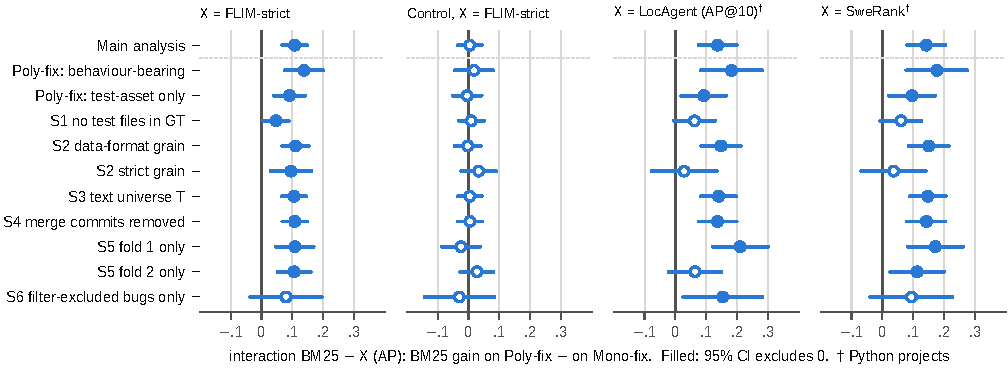
\includegraphics[width=\textwidth]{figures/fig_sensitivity.pdf}
\caption{RQ4 interaction (BM25's gain over technique X on Poly-fix bugs minus its gain on Mono-fix bugs, AP) under each sensitivity condition, with 95\% confidence intervals; the same values as the paper's sensitivity table.}
\end{figure}
\end{document}
